\section{Charge Carriers and Doping}

\subsection{Introduction}
We start learning about resistors, capacitors, and inductors from earlier courses such as EECS 16A and 16B. With more components like transistors, diodes, and op-amps (which are all based on semiconductors), we are able to expand upon circuit design. We need to understand semiconductor physics in order to understand how these components operate.
\begin{center}
    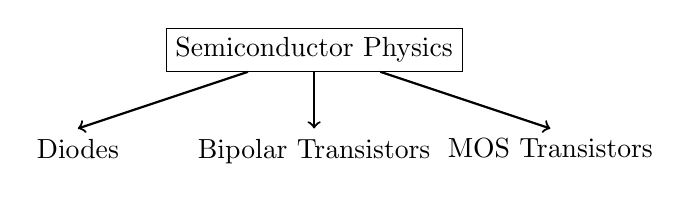
\begin{tikzpicture}
        \node[draw, align=center] (text) {Semiconductor Physics};
        \draw[->, thick] (text) -- ++(0,-1) node[below] {Bipolar Transistors};
        \draw[->, thick] (text) -- ++(-3,-1) node[below] {Diodes};
        \draw[->, thick] (text) -- ++(3,-1) node[below] {MOS Transistors};
    \end{tikzpicture}
\end{center}

We can also redefine Ohm's Law which we know as ($V = IR$) as $J = \sigma \vb{E}$. We can also write resistance($R$) and conductance($G$) in terms of other variables
\begin{gline}
    \item $J$: current density, $A/m^2$ (Amperes per meter squared)
    \item $\sigma$: conductivity, $S/m$ (Siemens per meter)
    \item $\vb{E}$: electric field, $V/m$ (Volts per meter)
\end{gline}

$R = \frac{R}{I} = \rho \frac{l}{A}$ and $G = R^{-1} = \sigma \frac{A}{l}$
\begin{gline}
    \item $\sigma$: conductivity
    \item $\rho$: resistivity
\end{gline}

For collisions in gas, we focus on the idea that initial velocity and direction is lost/randomized after a few collisions. So, when we sum over the random velocities of the particles and average it, it comes out to zero. Average momentum gain is:
\[\bar{\mu} = \frac{\vb{E} q \tau}{M} = \mu \vb{E}, ~~~ \mu := \frac{q \tau}{M} = \frac{\bar{v}}{\vb{E}}\]
\begin{gline}
    \item $\mu$: mobility, $m^2/ (V \cdot s)$
    \item $q$: electric charge, $1.60 \times 10^{-19}$, Coulombs = Amperes/second
    \item $\tau$: mean free time
    \item $M$: mass
    \item $\bar{v}$: average velocity
\end{gline}

Different elements have a different number of outer shell electrons. For semiconductors like silicon, we can increase the temperature to increase its conductivity. Silicon atoms are arranged in a diamond structure and in general, the energy levels that an atom can occupy are discrete. The \textbf{valence band} electrons are at a lower energy state (bound to host atoms) while \textbf{conduction band} electrons are at a higher energy state and are "free" electrons. These electrons are free to move around the crystal and take part in conduction. 

\subsection{Conduction and Fermi Dirac Distribution}
Thermal energy is on average about $\sim 26~eV$ at room temperature How large the \textbf{band-gap}, the gap between the conduction and valence band, determines how conductive a material is:
\begin{itemize}
    \item Insulators: band gap $\sim$ 15 $eV$
    \begin{itemize}
        \item Glass, rubber, oil, plastic, diamond
    \end{itemize}
    \item Semiconductors: band gap $\sim 1 eV$
    \begin{itemize}
        \item Silicon = 1.12 $eV$
    \end{itemize}
    \item Conductors: Not applicable due to overlapping conduction/valence bands
\end{itemize}
Because electrons are a type of particle called a \textbf{fermion}, we can say that 
\[f(\epsilon) = \frac{1}{e^{\frac{E - E_F}{k_B T}} + 1}\]
\begin{gline}
    \item $f(\epsilon)$: occupational probability of a state energy $\epsilon$
    \item $E_F$: fermi energy, $eV$
    \item $k_B$: Boltzmann's constant, $1.380649 \times 10^{-23} J/K$ (Joules per Kelvin)
    \item $T$: temperature in Kelvin
\end{gline}
\subsection{Doping}
\textbf{Doping} is defined as introducing impurities inside a silicon crystal to adjust the number of free electrons that we have. The following materials are commonly used:
\begin{pline}
    \item Group III elements: boron, aluminum, gallium $\rightarrow$ acceptors
    \item Group IV elements: germanium and silicon
    \item Group V elements: phosphorus, arsenic, antimony $\rightarrow$ donors
\end{pline}
Sometimes we assume that the number of electrons we add is much greater than the original free electrons that pure silicon had ($10^{10}$ per cubic centimeter). This leads to the simplification that the number of free electrons in our silicon crystal is $N_D$, where $N_D$ is the number of donor atoms that we add per cubic centimeter.

\subsection{Practice Problems}

\subsection{Sources}
\begin{itemize}
    \item \href{https://www.youtube.com/watch?v=yQDfVJzEymI}{\textcolor{blue}{Razavi Electronics 1, Lec 1, Intro., Charge Carriers, Doping}}
    \item \href{https://file.notion.so/f/f/048d6522-202b-48d4-b5d9-bc005bd602e2/214bf1f0-292f-48d6-9016-737d9f5da155/ee105_reader_v3.pdf?id=237a4300-3dbe-47d1-888b-ffae90d8352b&table=block&spaceId=048d6522-202b-48d4-b5d9-bc005bd602e2&expirationTimestamp=1714435200000&signature=yx-H1qvZJIodPfazOpwXX0Ce2mWMG8skOHl45xoPxus&downloadName=ee105_reader_v3.pdf}{EE105 Reader}
    \item Sedra, Adel S., et al. Microelectronic Circuits. Oxford University Press, 2021
    \item \href{https://eng.libretexts.org/Bookshelves/Materials_Science/TLP_Library_II/22%3A_Introduction_to_Semiconductors/22.2%3A_The_FermiDirac_Distribution}{Engineering LibreTexts: The Fermi-Dirac Distribution}
\end{itemize}

